\StartPlate{V23}{Two six-dimensional refinements with different signs}{The alternating form and dimension do not determine the Arf invariant.}
\begin{center}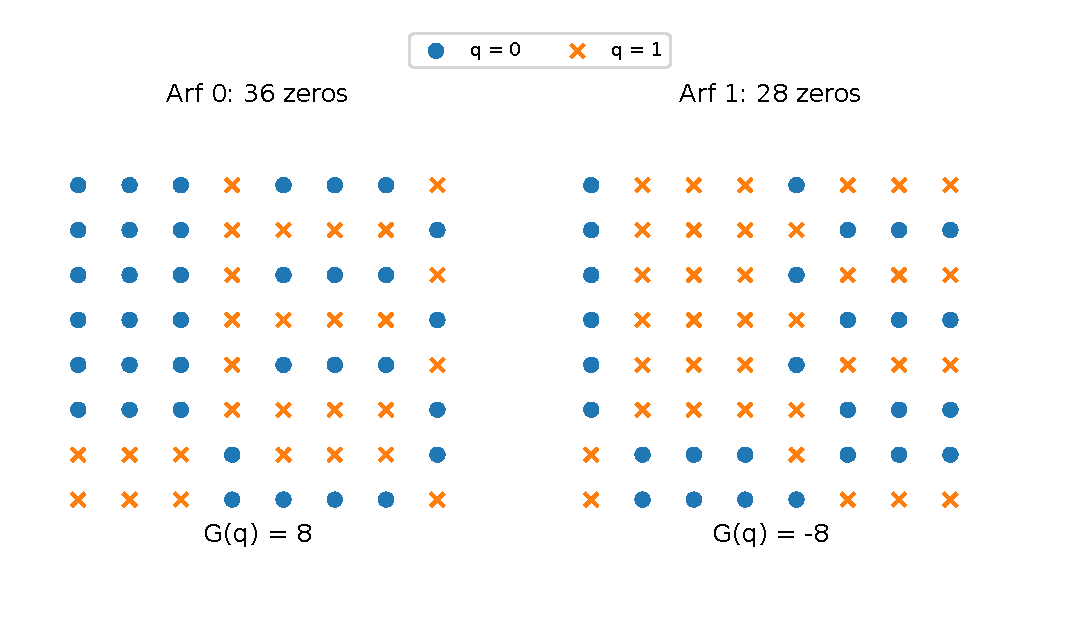
\includegraphics[width=\linewidth]{figures/V23.pdf}\end{center}
Each grid contains all $64$ binary vectors in dimension six. Columns encode the lower three bits and rows the upper three bits, with row zero at the top. Circles have quadratic value zero. Crosses have value one. The two forms share the standard polarization:
\[
q_+=x_1y_1+x_2y_2+x_3y_3,
\qquad q_-=q_++x_1+y_1.
\]
Their Gauss sums are $+8$ and $-8$. Consequently the zero counts, including the zero vector, are $(64+8)/2=36$ and $(64-8)/2=28$. The diagrams use exact binary evaluation at every vector.

These are explicit abstract refinements, not a claim that either has been computed on the actual rank-eight arithmetic candidate. The example shows the datum still required when the host marking is independently fixed. At equal capacity, an Arf mismatch has no orthogonal complement in which to be absorbed.
\vfill\PlateSource{Exhaustive 64-vector displays}{Part III, Section 27.1}{69}
